% !TEX root = SegwayDoku.tex
\renewcommand{\autoren}{Valentyn Chepil}
\newpage
\section{Die ausgewählte Komponentenliste}
\subsection{Die Motoren}

% bild und Modul-Name

\subsection{Endcoder}

\begin{figure}[!h]  % [h] bedeutet, dass das Bild genau an dieser Stelle im Text erscheint
	\centering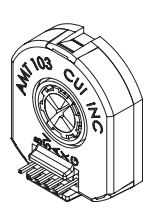
\includegraphics[width=0.3\textwidth]{images/Entcoder.jpg}
	% caption ist die Bildunterschrift, taucht auch im Abbildungsverzeichnis auf
	\caption{AMT103-V  \newline (Quelle: cui.com )}
	\label{Endcoder} % über das label kann man aus dem Text auf das Bild verweisen
\end{figure}

Model: AMT103-V
% bild und Modul-Name

\subsection{Driver}

% bild und Modul-Name

\subsection{Steuerungsplatine}
\begin{figure}[!h]  % [h] bedeutet, dass das Bild genau an dieser Stelle im Text erscheint
	% mit width=... wird die Größe des Bildes in Prozent der Seitenbreite eingestellt
	\centering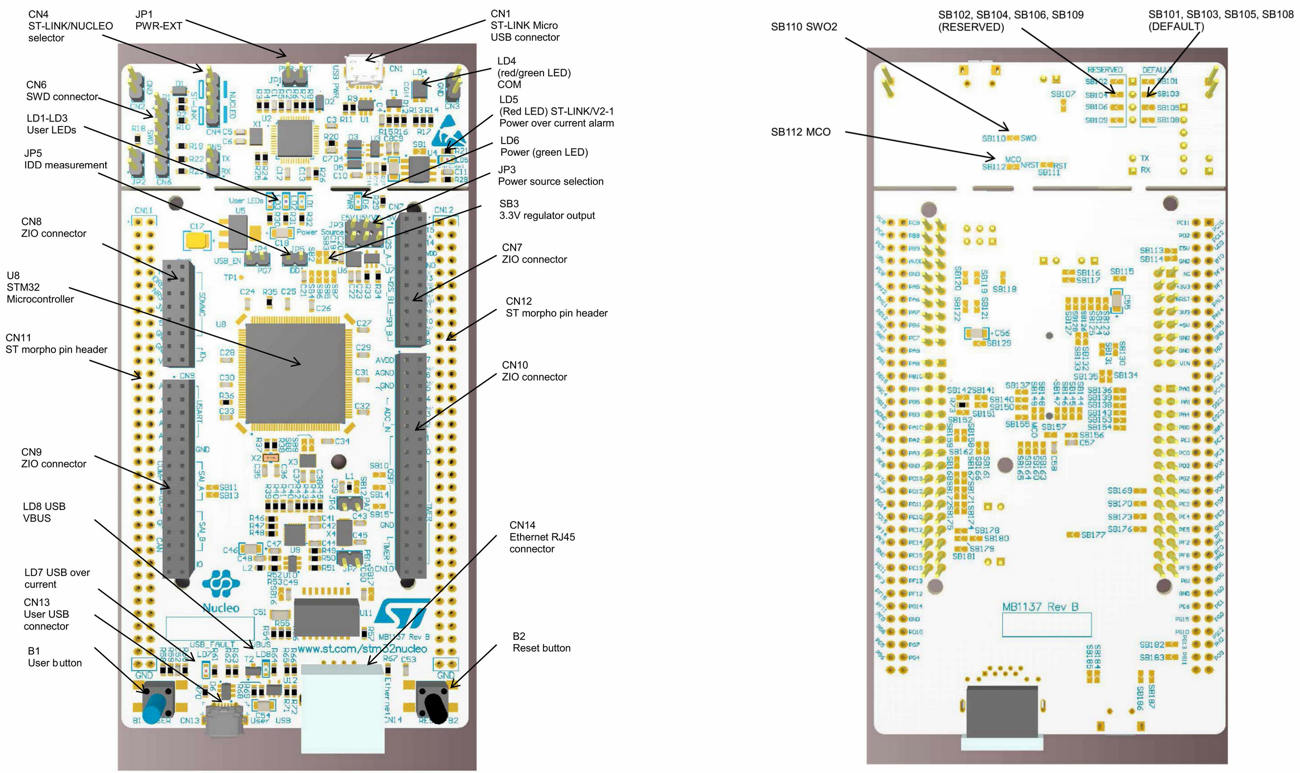
\includegraphics[width=0.8\textwidth]{images/Nucleo.jpg}
	% caption ist die Bildunterschrift, taucht auch im Abbildungsverzeichnis auf
	\caption{Nucleo-F746ZG  \newline (Quelle: playembedded.org )}
	\label{Nucleo} % über das label kann man aus dem Text auf das Bild verweisen
\end{figure}



\subsection{Die Räder}

\begin{figure}[!h]  % [h] bedeutet, dass das Bild genau an dieser Stelle im Text erscheint
	% mit width=... wird die Größe des Bildes in Prozent der Seitenbreite eingestellt
	\centering\includegraphics[width=0.5\textwidth]{images/reifen.png}
	% caption ist die Bildunterschrift, taucht auch im Abbildungsverzeichnis auf
	\caption{Reifen \newline (Quelle: www.haertle.de )}
	\label{reifen} % über das label kann man aus dem Text auf das Bild verweisen
\end{figure}

quelle:
https://www.haertle.de/RC+Modellbau/RC+Car+Zubehoer/Reifen+Felgen+Raeder/TAMIYA+54188+DB+01+Dual+Block+Reifen+C+hinten+62+35.html
% bild
Felgen werden 3D moduliert und gedruckt. (In der Gruppe abfragen)

\subsection{Die Hinderniserkenner}

% bild und Modul-Name

US-Sensor und Infrarot-Sensor

\subsection{Bewegungs- und Beschleunigungsaufnehmer }

Hyroskop Modul-Name und Bild

\subsection{Netz (Akku)}

 Name und Bild
 
 \subsection{...}
 
 Name und Bild

